\documentclass{qbook}
\addbibresource{bib/Reference.bib}  % 导入参考文献数据库
\begin{document}
\setcounter{page}{-1} % 设置计数为-1, 确保正文从0开始
%# -*- coding: utf-8-unix -*-
\thispagestyle{empty}
\begin{tikzpicture}[overlay,remember picture,font=\sffamily\bfseries]
	\draw[ultra thick,c4,name path=big arc] ([xshift=-2mm]current page.north) arc(150:285:11)
	coordinate[pos=0.225] (x0);
	\begin{scope}
		\clip ([xshift=-2mm]current page.north) arc(150:285:11) --(current page.north
		east);
		\fill[c4!50,opacity=0.25] ([xshift=4.55cm]x0) circle (4.55);
		\fill[c4!50,opacity=0.25] ([xshift=3.4cm]x0) circle (3.4);
		\fill[c4!50,opacity=0.25] ([xshift=2.25cm]x0) circle (2.25);
		\draw[ultra thick,c4!50] (x0) arc(-90:30:6.5);
		\draw[ultra thick,c4] (x0) arc(90:-30:8.75);
		\draw[ultra thick,c4!50,name path=arc1] (x0) arc(90:-90:4.675);
		\draw[ultra thick,c4!50] (x0) arc(90:-90:2.875);
		\path[name intersections={of=big arc and arc1,by=x1}];
		\draw[ultra thick,c4,name path=arc2] (x1) arc(135:-20:4.75);
		\draw[ultra thick,c4!50] (x1) arc(135:-20:8.75);
		\path[name intersections={of=big arc and arc2,by={aux,x2}}];
		\draw[ultra thick,c4!50] (x2) arc(180:50:2.25);
	\end{scope} 
%	\path[decoration={text along path,text color=c4,
%		raise = -2.8ex,
%		text along path,
%		text = {|\sffamily\bfseries|\today},
%		text align = center,
%	},
%	decorate
%	] ([xshift=-2mm]current page.north) arc(150:245:11);
	%
	
	\begin{scope}
		\path[clip,postaction={fill=c3}]
		([xshift=2cm,yshift=-8cm]current page.center) rectangle ++ (4.2,7.7);
		\fill[c2] ([xshift=0.5cm,yshift=-8cm]current page.center)
		([xshift=0.5cm,yshift=-8cm]current page.center)  arc(180:60:2)
		|- ++ (-3,6) --cycle;
		\draw[ultra thick,c4] ([xshift=-1.5cm,yshift=-8cm]current page.center) 
		arc(180:0:2);
		\draw[ultra thick,c4] ([xshift=0.5cm,yshift=-8cm]current page.center) 
		arc(180:0:2);
		\draw[ultra thick,c4] ([xshift=2.5cm,yshift=-8cm]current page.center) 
		arc(180:0:2);
		\draw[ultra thick,c4] ([xshift=4.5cm,yshift=-8cm]current page.center) 
		arc(180:0:2);
		\fill[red] ([xshift=2.5cm,yshift=-8cm]current page.center) +(60:2) circle(1.5mm);
		\node[text=c5!80!black] at ([xshift=4.7cm,yshift=-5.2cm]current page.center) {$\rho:=\dfrac{1+\sqrt{-3}}{2}$};
	\end{scope}
	%
	\fill[c1] ([xshift=2cm,yshift=-8cm]current page.center) rectangle ++ (-13.7,7.7);
	\node[text=white,anchor=west,scale=4,inner sep=0pt] at
	([xshift=-10.55cm,yshift=-2.5cm]current page.center) {拟稳定耗散系统};
	\node[text=white,anchor=west,scale=4,inner sep=0pt] at
	([xshift=-10.55cm,yshift=-4.5cm]current page.center) {动力学};
	\node[text=white,anchor=west,scale=1.5,inner sep=0pt] at
	([xshift=-4.5cm,yshift=-5.8cm]current page.center) {Igor Chueshov};
	\node[text=white,anchor=west,scale=1.5,inner sep=0pt] at
	([xshift=0cm,yshift=-5.8cm]current page.center) {著};
	\node[text=white,anchor=west,scale=1.5,inner sep=0pt] at
	([xshift=-4.5cm,yshift=-6.8cm]current page.center) {沈卓洋};
	\node[text=white,anchor=west,scale=1.5,inner sep=0pt] at
	([xshift=0cm,yshift=-6.8cm]current page.center) {译};
\end{tikzpicture}
\clearpage
\thispagestyle{empty}
\begin{center}
	\Large{\sffamily\bfseries\heiti 编译日期: \today} 
	\vspace{1em}\\
	\Large{\sffamily\bfseries\heiti 任何建议及错误信息请发送至邮箱}\\
	\texttt{shenzhy2020@lzu.edu.cn}
\end{center} 
\vfill
\vspace{30em}
\begin{tabular*}{\textwidth}{ccc}
	\includegraphics{figure/by-nc.eps}
	& \begin{minipage}[b]{0.6\textwidth}
		\small\sffamily
		本作品采用知识共享 署名-非商业性使用 4.0 国际 许可协议进行许可. 访问\url{http://creativecommons.org/licenses/by-nc/4.0/}查看该许可协议.
	\end{minipage}
\end{tabular*}  % 载入封面
%\watermark{45}{10}{draft}
%======================================================================
\frontmatter  % 对前言和介绍等用罗马数字作为页码
\include{tex/mypreface} % 前言
\begin{PreChapter}{原书前言}
	本书的主要目的是介绍无穷维演化模型的背景和最新发展的数学研究方法, 考虑各种形式和来源的耗散性和稳定性. 
	
	耗散系统的主要特征是存在更高阶的衰减这种能量重新分配机制, 这种机制可以导致系统中复杂的极限状态和结构的产生, 它在某些情况下是稳定的. 人们普遍认为, 20世纪80年代在寻找合适的能够解释湍流现象的数学模型的过程中, 耗散系统的一般理论得到了显著发展. 至今, 无穷维耗散系统的研究已经取得了显著进展(见例如以下专著\cite{Babin92}, \cite{Chepyzhov02}, \cite{Hale88}, \cite{Ladyzhenskaya91}, \cite{Robinson01}, \cite{Sell02}, \cite{Temam97}和它们的参考资料). 
	
	相较于其他提及的材料, 本书的主要特点是系统性的介绍、发展和利用了拟稳定的方法, 这种方法是和Irena Lasiecka在\cite{Chueshov08}, \cite{Chueshov10}(亦可见最新的研究\cite{Chueshov13})中合作的, 它最初被设计用于二阶非线性阻尼模型. 这里我们大幅扩展了这个方法, 更多种类的二阶方程、抛物模型以及迟滞偏微分系统也将被包括在考虑范围之内. 
	
	我们希望本书不仅对对动力系统的一般理论感兴趣的数学工作者有帮助, 也可以对对连续介质力学中出现的无穷维耗散系统的渐近分析的数学背景和方法感兴趣的物理学家和工程师有用. 
	
	我们的介绍基于一般和抽象的模型, 涵盖了几个重要的生成无穷维耗散系统的非线性偏微分方程种类, 它们包括热以及反应扩散模型、用于研究湍流现象的二维流体动力学中出现的广泛模型和具有非线性状态依赖阻尼的板波模型, 我们还考虑了非线性阻尼波Kirchhoff模型和一些抛物和双曲类型的时滞问题. 
	
	本书中的大部分分析都致力于动力学的稳定性, 以及将无限维系统严格简化为某些有限维结构, 这些结构仅通过有限多个自由度来刻画. 这些有限维结构应该引起应用型科学家的兴趣, 他们追求现实的无穷维现象的数学模拟. 
	
	本书包括大量的习题, 正如Dan Henry著名的专著\cite{Henry81}那样, 它们是本书不可或缺的一部分, 它们中的大多数被策略性地放置在文本中, 而不是放在一个部分的末尾, 一些习题是常规的, 而另外一些习题则是以“习题”形式编写的一般的评论和注解, 这使得我们能够缩短叙述以及避免额外的细节. 
	
	本书可以作为研究生阶段耗散动力学课程的教材. 了解泛函分析和常微分方程的基本概念和事实就足以理解本书.  事实上, 本书的许多部分已经在作者在Kharkov大学开设的高级本科和研究生课程中使用过. 

	\section*{致谢}

	我很高兴向所有帮助我理解耗散动力学本质的同事表示感谢. 我最衷心的感谢Irena Lasiecka, 我们在非线性偏微分方程动力学方面进行了许多非常启发性的讨论和愉快的合作. 我要感谢Alexander Rezounenko对状态依赖时滞模型的评论和富有成效的讨论. 感谢我的儿子Gennadiy在绘制所有插图时的慷慨帮助, 感谢我的妻子Galina对我在创作本书时长久的鼓励. 我还要感谢Springer出版社的编辑们(尤其是Donna Chernyk)对这个项目的关心和值得赞赏的帮助. 在自2014年春季初稿开始创作的过程中, 我收到了相当多匿名审稿人的11条(十一条!)意见, 感谢他们的宝贵意见和建议. 
		
	\vspace{1em}
	\begin{flushright}
		\begin{minipage}{0.3 \textwidth}
			\begin{tabular}{c}
				{Igor Chueshov} \\
				2015年6月于Kharkov, Ukraine
			\end{tabular}
		\end{minipage}
	\end{flushright}

\end{PreChapter}	
	
	 % 原作前言
\tableofcontents % 目录
\begin{PreChapter}{介\quad 绍}
	动力系统的一般理论起源于常微分方程,其基础由H. Poincaré(1854–1912)和A.M. Lyapunov(1857–1918)奠定。G.D. Birkhoff(1884–1944)对该理论作出了重要贡献,他是“动力系统”一词的提出者,并且利用了拓扑的方法,在抽象的层次很大程度的发展了动力系统理论。动力系统的概念是一般的科学上的演化(依赖于时间)过程概念的数学化,这些过程可以是相当不同的自然现象。动力系统自然地诞生于对物理、化学、生物、生态、经济,甚至社会现象的研究。动力系统的概念包括一个可能的状态的集合(相空间),以及状态关于时间的演化法则。因此,“动力系统”这一概念覆盖了相当多模型的种类,只要这些模型也许能描述任意对象关于时间的演化和依赖于时间的过程。例如,这些对象和过程包括由在连续介质力学和数学物理中产生的非线性演化偏微分方程生成的模型。这些模型需要无穷维空间用以表示各种可能的状态。在本书中,我们专注于(无穷维)系统,这些系统展示了各种类型的能量迁移和耗散。似乎(见,例如\cite{Hale88},\cite{Raugel02},\cite{Temam97}中的讨论)这些作用在\cite{Levinson45}的文章中被严格定义,该文章以现代(数学)的形式介绍了(动力学的)耗散性的概念;也可见\cite{Billoti71},\cite{Coddington55},\cite{Pliss66},\cite{Pliss77}。耗散性意味着动力学行为在相空间中被局部化。这可以被表达为关于有界吸收集存在性的陈述。在具有有限自由度的系统的情形中,这种局部化允许我们选择限制性对象,例如吸引子,它含有关于系统稳定性的重要信息。无穷维系统的情况会变得非常不同。为了挑选出相应的限制机制,我们需要额外的演化的紧致性条件。这使得无穷维的理论变得更加复杂。尽管如此,到目前为止,集中关注不同类型的PDE模型,无穷维动力系统理论的几个重要的方面已经得到了发展(见,例如这些专著\cite{Babin92},\cite{Chepyzhov02},\cite{Chueshov99},\cite{Chueshov10},\cite{Chueshov08},\cite{Hale88},\cite{Ladyzhenskaya91},\cite{Robinson01},\cite{Sell02},\cite{Temam97},以及这些研究\cite{Babin06},\cite{Miranville08},\cite{Raugel02})。
	
	本书聚焦于无穷维耗散动力系统。为了将理论的一般化达到合理的程度,我们的考虑是相对抽象的,并且协调了各种在抽象空间上定义的一般的演化方程。我们的目标是介绍与基本的动力系统长时间行为有关性质的一般方法和抽象结果。我们的主要工具是基于耗散系统相关的拟稳定性质。粗略的讲,拟稳定性意味着我们可以通过将两条轨道的差异分解为收敛部分和紧致部分来控制轨道的发散。
	
	本书的主要特点(相较其他书籍)有以下几个方面:

	\begin{itemize}
		\item 我们展示、发展和阐述了一种基于相对较新的观察的动力系统紧性的方法,它在\cite{Khanmamedov06}被提出(亦可见\cite{Chueshov08}和\cite{Chueshov10}),并且已经被证明在临界非线性问题的研究中非常有效。这种方法在势能的辅助下,作为二阶演化方程的补偿紧性方法出现,并且已经被应用到许多其他情形中。事实上,这种方法展示了一种拟稳定性的弱形式。
		
		\item 为了研究关于有限维吸引子和它的光滑性的问题,我们促成和发展了一种关于一些二阶演化方程拟稳定性的全新方法,它最初在\cite{Chueshov04}中被介绍(亦可见\cite{Chueshov08}和\cite{Chueshov10}以及最近的研究\cite{Chueshov13})。这种方法的主要优势是可以将对动力系统的初始的光滑性的要求降到最低。
		
		\item 在本书中,我们非常注重将理论应用于无限维系统,这些系统源自于连续介质力学和数学物理。然而,为了使抽象方案更加透明并呈现复杂行为的不同可能场景,我们集中使用了低维的ODE作为例子, 其中一些是真实世界PDE模型的低程度的近似。
		
		\item 我们提供了适用于无穷维(局部紧)情形的现代形式的动力系统理论的基本概念,部分素材我们以练习题的形式给出。其中一部分练习题提供了有关所考虑对象的额外信息,这使得文本更加集中,事实上,许多练习题可以“练习”的标题替换成例如“容易见得”这样的文本。但是,我们更倾向于使他们保持“量化”的形式,并且我们相信,这会使得内容更加友好。
	\end{itemize}

	本书的组织方式如下:

\end{PreChapter} % 介绍
%======================================================================
\mainmatter	  % 对正文用阿拉伯数字作为页码
\pagestyle{fancy} % 设置页眉页脚
\chapter{基本概念}\label{cpt:1}

本章收集了一般的动力系统理论中的基本定义、概念和最简单的说明性陈述. 我们还描述了所有1维和2维连续动力系统的可能场景, 并通过例子讨论了主要的分歧图像. 我们后半部分叙述的主要目的是, 给读者以低维(1或2维)的连续时间演化算子会产生什么样动力学行为的感觉.

我们主要遵循\cite{Nemytskii60}和\cite{Sibirsky75}的表述方式, 并且依赖经典的常微分材料; 见\cite{Coddington55}, \cite{Hartman02}, \cite{Lefschetz77}以及\cite{Bautin90}和\cite{Reissing74}.

\section{演化算子和动力系统}
如同介绍中已经提及的, 动力系统的概念包括可能出现的状态的集合(相空间)和状态关于时间的演化法则. 在之后的叙述中, 我们选取完备的度量空间作为相空间, 记$\mathbb{T}_{+}$为$\mathbb{T}$上的非负元素用以代表时间, 其中$\mathbb{T}$为$\mathbb{R}$或$\mathbb{Z}$.

\begin{definition}{演化算子}{EO}\index[word]{yanhuasuanzi@演化算子(evolution operator)}\index[symbol]{$S_{t}$}
	设$X$是完备的度量空间, $\mathbb{T}=\mathbb{Z}$或$\mathbb{R}$, 对任意$t\in\mathbb{T}$, $S_{t}:X\mapsto X$是连续映射, 并且满足半群性质, 即:$$S_{0}=id_{X},\quad S_{t+\tau}=S_{t}\circ S_{\tau},\quad\forall t,\tau\in\mathbb{T}^{+},$$则称$\{S_{t}\}_{t\in \mathbb{T}^{+}}$为演化算子(或演化半群、半流). 
\end{definition}

在$\mathbb{T}=\mathbb{R}$的情形中, 我们额外假设映射$t:\mapsto S_{t}x$是$\mathbb{R}_{+}$到$X$上关于$x$的连续映射.  我们称$(X,S_{t})$为相空间为$X$、演化算子为$S_{t}$的\textbf{动力系统}. 

在$\mathbb{T}=\mathbb{Z}$时, 演化算子(以及动力系统)被称为离散(或关于离散时间)的.  如果$\mathbb{T}=\mathbb{R}$, 则$S_{t}$(同理, $(X,S_{t})$)被称为关于时间连续的演化算子(动力系统). 如果相空间可以被定义维数(例如, 当$X$为线性空间时), 则$\dim X$被称为动力系统的维数. 

接下来以一个例子来说明\rdef{def:EO}. 

\begin{example}{常微分方程}{ODE}
	设$F:\mathbb{R}^{d}\mapsto\mathbb{R}^{d}$为(非线性)映射. 考虑方程
	\begin{equation}\label{equ:exa1}
		\frac{\mathrm{d}u(t)}{\mathrm{d}t}=F(u(t)),\quad t\geqslant 0,\quad u(0)=u_{0}\in\mathbb{R}^{d}.
	\end{equation}
	如果对任意初始点$u_{0}\in\mathbb{R}^{d}$, 这个问题都有依赖于$u_{0}$的唯一解, 则它在$X=\mathbb{R}^{d}$上, 以$S_{t}u_{0}=u(t,u_{0})$的形式生成了一个演化半群, 其中$u(t,u_{0})$是问题\requ{equ:exa1}的解. 于是, 我们得到了相空间$X=\mathbb{R}^{d}$上的动力系统$(X,\mathbb{R}^{d})$. 
\end{example}

\begin{example}{映射}{MP}
	设$X$是完备的度量空间. 考虑映射$F:X\mapsto X$. 令$n\in\mathbb{Z}_{+}$, 则$F$的$n$重复合$S_{n}\equiv F\circ\cdots\cdots F$形成了一个演化算子序列$\{S_{n}\}_{n=0}^{\infty}$. 如果$F$是连续映射, 则我们得到了一个离散的动力系统$(X,S_{n})$. 
\end{example}

在\rexa{exa:MP}中, $(X,F)$完全地决定了(离散)动力系统$(X,S_{n})$, 因此$(X,F)$也经常被叫做动力系统. 接下来的例子展示了如何通过单个映射来生成一个连续时间的动力系统. 

\begin{example}{映射生成的连续时间系统}{CTS}
	和\rexa{exa:MP}一样, 设$X$是完备的度量空间, 并且$F:X\mapsto X$是连续映射. 考虑连续参数的微分方程$$u(t+1)=F(u(t)),\quad t\in\mathbb{R}_{+}.$$这个方程的任意解都可以轻易地通过定义在$[0,1]$上的函数$\phi(\xi)$, 以以下形式来构造, $$u(t)=S^{n}(\phi(t-n)),\quad n\leqslant t<n+1,\quad n\in\mathbb{Z}_{+},$$其中$S_{n}\equiv F\circ\cdots\circ F$. $u$在$\mathbb{R}_{+}$上是连续的, 当$$\phi\in Y=\{\phi\in C([0,1],X):\phi(1)=F(\phi(0))\},$$其中$C([0,1],X)$是$[0,1]$到$X$的连续函数. 现在我们可以通过以下形式来定义$Y$中的连续时间演化算子$$S_{t}:\phi(\xi)\mapsto F^{[t+\xi]}(\phi(\{t+\xi\})),\quad t\in\mathbb{R}_{+},$$其中$[\xi]$是$\xi$的整数部分, $\{\xi\}$是$\xi$的小数部分. 
\end{example}

在\rexa{exa:CTS}中, 我们得到了一个连续时间的系统$(Y,S_{t})$. 这种类型的系统(主要是$X$是$\mathbb{R}$上的区间的情形)在\cite{Sharkovsky86}中有密集讨论; 亦可见\cite{Sharkovsky89}. 动力系统$(Y,S_{t})$的特点提供了最近被介绍和发展的理想湍流的概念的动机; 见\cite{Sharkovsky06}. 

\begin{example}{Bebutov动力系统}{BDS}\index[word]{Bebutovdonglixitong@Bebutov动力系统(Bebutov dynamical system)}\index[word]{Bebutovduliang@Bebutov度量(Bebutov metric)}
	设$X=C(\mathbb{R})$为所有$\mathbb{R}$上的连续函数以Bebutov度量构成的空间, 其中Bebutov度量定义为$$\mathrm{dist}(\psi,\phi)=\sup_{r>0}\min\left\{\sup_{|x|\leqslant r}|\psi(x)-\phi(x)|,\frac{1}{r}\right\}.$$在这种情况下, $X$成为一个完备的度量空间, 并且在Bebutov度量意义下的收敛等价于有界集上的一致收敛(见, 例如\cite{Sibirsky75}). 我们以左平移算子为演化算子$$(S_{t}f)(x)=f(x+t),\quad f\in X,\quad t\geqslant 0.$$
\end{example}

\rexa{exa:BDS}中的系统$(X,S_{t})$被称为Bebutov(平移)动力系统. 在这个系统的帮助下, 我们很容易展示不同种类的独立轨道的动力学(见, 例如\cite{Nemytskii60},\cite{Sibirsky75}和它们的参考文献). 

\begin{remark}{闭算子\footnote{我们推荐初学者略过此注记}}{CEO}
	许多动力学的一般性质不需要假设演化算子$S_{t}$的连续性, 这对研究一些无穷维偏微分方程模型很重要. 根据\cite{Pata07}, 我们可以假设演化算子$S_{t}$在相应的空间$X$下是闭的, 来代替$S_{t}$的连续性要求. 这意味着, 对任意$t>0$, 在$n\to\infty$时$x_{n}\to x, S_{t}x_{n}\to y$, 则$S_{t}x=y$, 显然$S_{t}$的连续性可以得到闭性. 然而, 逆命题仅在一些额外条件下成立, 即可以证明如果$S_{t}$是闭的, 并且把任何紧集映成相对紧集, 则$x\mapsto S_{t}$是连续的. 的确, 设在$n\to\infty$时$x_{n}\to x$, 对任意$t>0$我们可以选择子列$\{n_{m}\}$, 使得$S_{t}x_{n_{m}}\to y$. 由$S_{t}$的闭性知, $S_{t}x=y$, 进一步, $\{S_{t}x_{n}\}$除了$y=S_{t}x$以外没有其他极限点, 这意味着$S_{t}$的极限性. 另一方面, 映射$$f(x)=\begin{cases}(1-x)^{-1},&\quad 0\leqslant x<1;\\x,&\quad x\geqslant 1,\end{cases}$$是一个闭算子但不是连续的(其他例子见\cite{Pata07}). 闭演化算子产生于一类状态依赖的时滞偏微分方程系统的长时间动力学的研究(见\ref{sec:6.2}).
	
	我们还注意到, 算子的闭性是(无界)线性算子理论中众所周知的概念, 见例如\cite{Dunford58}的第二章或\cite{Yosida74}的第二章. 我们知道, 演化算子语境中的闭性概念, 在\cite{Babin92}中作为(强连续)演化半群的(弱)闭性(亦可见\cite{Chueshov99}和下面的\rthm{thm:})和\cite{Pata07}中的一般情形出现. 
\end{remark}

在定性行为的研究中, 动力系统的等价概念发挥着重要的作用. 这种等价关系使我们能够将广泛的动力系统划分成各种具有非常相似行为的系统. 

\begin{definition}{拓扑等价}{TE}\index[word]{tuopudengjia@拓扑等价(topology equivalence)}\index[word]{tonggou@同构(isomorphic)}
	设$(X,S_{t})$和$(\tilde{X},\tilde{S}_{t})$为两个动力系统, 如果存在同胚映射$h: X\cong\tilde{X}$的, 使得对任意$x\in X$和$t\in\mathbb{T}_{+}$, 都有$$
	h(S_{t}x)=\tilde{S}_{t}h(x),$$则称动力系统$(X,S_{t})$和$(\tilde{X},\tilde{S}_{t})$\textbf{拓扑等价}(或\textbf{同构}), 记作$(X,S_{t})\cong (\tilde{X},\tilde{S}_{t})$.  此时称演化算子$S_{t}$与$\tilde{S}_{t}$\textbf{拓扑共轭}.  
\end{definition}

\begin{exercise}
	设$h$是使得$(X,S_{t})$和$(\tilde{X},\tilde{S}_{t})$拓扑等价的同胚映射, 则$h^{-1}$亦是.
\end{exercise}

\begin{proof}
	由$h^{-1},(h^{-1})^{-1}=h$的连续性知, $h^{-1}$是同胚映射. 任取$\tilde{x}\in \tilde{X}$, 由$h$是双射知, 存在$x\in X$使得$h(x)=\tilde{x}$, 那么对任意$t\in\mathbb{T}_{+}$, 有$$
	h^{-1}(\tilde{S_{t}}\tilde{x})=h^{-1}(\tilde{S_{t}}h(x))=h^{-1}h(S_{t}x)=S_{t}x=S_{t}(h^{-1}\tilde{x}).$$
\end{proof}

接下来用一个习题来说明\rdef{def:TE}. 

\begin{exercise}
设$\alpha,\beta>0$并且$\alpha,\beta\neq 1$, 则两个离散(?)系统(时间呢?)$(\mathbb{R}_{+},\alpha x)$和$(\mathbb{R}_{+},\beta x)$拓扑等价当且仅当$\alpha,\beta$同时大于$1$或小于$1$.
\end{exercise}

\begin{proof}
	必要性???: 设$(\mathbb{R}_{+},\alpha x)\cong (\mathbb{R}_{+},\beta x)$, 则存在同胚映射$h$, 使得$$
	h(\alpha x)=\beta h(x),$$
	
	充分性: 设$\alpha,\beta$同时大于$1$或小于$1$, 则$\log_{\alpha}\beta>0$, 于是$h(x):=x^{\log_{\alpha}\beta}:\mathbb{R}_{+}\cong \mathbb{R}_{+}$, 并且对任意$x\in\mathbb{R}_{+}$, 有$$h(\alpha x)=(\alpha x)^{\log_{\alpha}\beta}=\beta x^{\log_{\alpha}\beta}=\beta h(x),$$即$(\mathbb{R}_{+},\alpha x)\cong (\mathbb{R}_{+},\beta x)$
\end{proof}


\section{轨道, 不变集和平衡点}
现在我们来回忆一下动力系统理论中的几个著名概念(见, 例如)

\begin{definition}{不变集}{IS}
	设$S_{t}$是$X$.
\end{definition}


\section{Omega-极限集}
\section{独立轨道的极限性质}
\section{轨道的循环性质}
\section{平衡点与Lyapunov稳定性}
\section{$1$维连续系统的完整理论}
\section{二维系统定性行为的可能类型}
\section{分歧理论举例}

\chapter{耗散系统的基本事实}\label{cpt:2}
\chapter{有限维的行为和拟稳定性}
\chapter{抛物问题概述}
\chapter{二阶演化方程}
\chapter{无穷维空间的时滞方程}
\appendix % 之后是附录
\chapter{一些辅助事实}
\chapter{原书勘误表}
	\errPositon{第二页, 最后一行}{exa:CTS}
	\errOrig $$S_{t}:\phi(\xi)\to F^{[t+\xi]}(\phi(\{t+\xi\}),\quad t\in\mathbb{R}_{+},$$
	\errCorr $$S_{t}:\phi(\xi)\to F^{[t+\xi]}(\phi(\{t+\xi\})),\quad t\in\mathbb{R}_{+},$$	

\backmatter % 结束正文, 取消章节序号
%======================================================================
\printbibliography[heading=bibintoc] % 打印参考文献
\printindex[symbol] % 打印索引
\printindex[word] 
\makeatletter 
\makeatother
\end{document}